\documentclass[a4paper,12pt]{report}

%chargement des extensions requises au bon fonctionnement de l'extension et des documents
\usepackage[utf8x]{inputenc}
\usepackage[T1]{fontenc}
\usepackage[french]{babel}
\usepackage{graphicx}
\usepackage{lipsum}
\usepackage[a4paper]{geometry}
\usepackage{wallpaper}
\usepackage{libertine}
\usepackage{csquotes}
\usepackage{vmargin}
\usepackage{hyperref}
\usepackage[colorinlistoftodos]{todonotes}
\usepackage{titlesec}
\usepackage{array}
\usepackage{amsmath}
\usepackage{tikz}
\usepackage{pgfplots}
\usepackage[final]{pdfpages}


%Gestion des marges
\newgeometry{left=30mm,right=30mm,top=30mm,bottom=30mm}

% Suppressions des veuves et orphelines
\widowpenalty=10000
\clubpenalty=10000

% Suppressions de l'espace avant les chapitres
\titleformat{\chapter}[display]
{\normalfont\huge\bfseries}{\chaptertitlename\ \thechapter}{20pt}{\Huge}
\titlespacing*{\chapter}{0pt}{-20pt}{30pt}

%Type de colonne pour tableau
\newcolumntype{C}[1]{>{\centering\arraybackslash}m{#1}}

% Définition de l'affichage des sections (I.1 sans redondance)
\setcounter{secnumdepth}{2}
\renewcommand   \thesection         {\Roman{section}}
\renewcommand   \thesubsection      {\thesection.\arabic{subsection}}

% Each new section starts on a new page
\newcommand{\sectionbreak}{\clearpage}



\author{Gautier \textsc{Colajanni}, Cédric \textsc{Jezequel},\\ Julien \textsc{Marcou}, Pierre \textsc{Poilane}, Paul \textsc{Rivière}, Kévin \textsc{Thek}}

\title{Rapport de projet Acquisition de Connaissances \\ Authorship Attribution}

\begin{document}

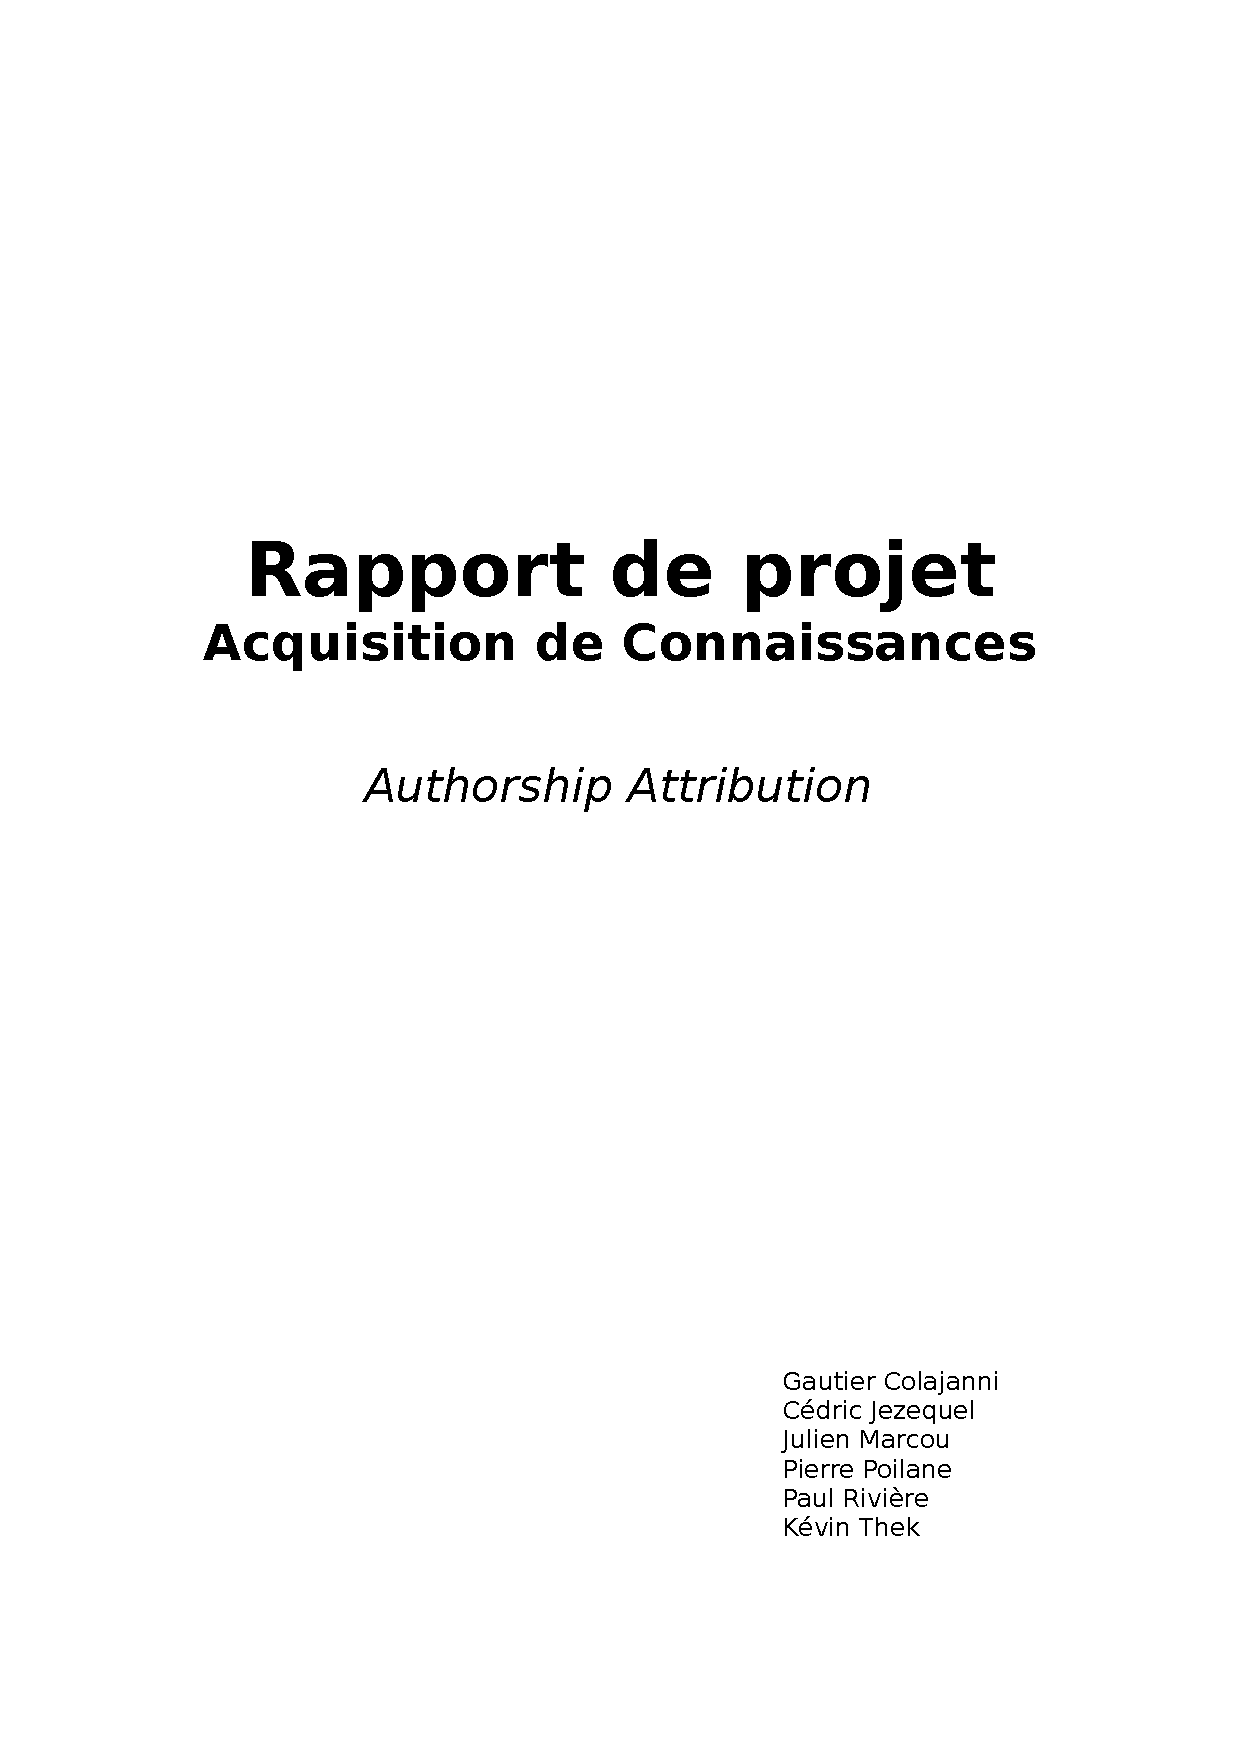
\includepdf{./garde.pdf}

% Insertion d'une page blanche
\newpage \thispagestyle{empty}
\null
\newpage 

% Sommaire
\renewcommand\contentsname{Sommaire}
\tableofcontents


\section*{Introduction}
\addcontentsline{toc}{section}{Introduction}

Étudiants à l'INSA Rennes, notre projet consiste à développer une chaîne logicielle permettant de mettre en œuvre des algorithmes de classification automatisée. Cette classification automatisée a pour sujet des documents textuels issue de la presse en langue anglaise. Par l'intermédiaire de nos implémentations, nous souhaitons réussir à deviner l'auteur d'un texte en ayant préalablement analysé son corpus.

Ce rapport traite des expérimentations que nous avons effectué sur diverses techniques de classification et nous permet de dresser un tableau des performances de chaque algorithme. Nous n'avons pas la prétention de parvenir à un classifieur optimal mais souhaitons parvenir à une solution fonctionnelle afin de sentir les difficultés et aspects de ces méthodes.

Nous avons divisé notre groupe en deux afin de réaliser deux analyses nous semblant différentes. La première technique consiste en une sélection de critères de discrimination uniquement basée sur les fréquences des termes utilisés par les auteurs. La deuxième méthode va s'orienter sur la nature des mots employé et la construction des phrases pour identifier l'auteur par son style. Ces deux sous-projets sont ensuite comparés afin de montrer les difficultés rencontrées et les performances que nous avons été capables d'atteindre.

\subsection*{Détails techniques}

Notre projet portant s'effectuant en un temps restreint et souhaitant obtenir des résultats rapidement sans avoir à capitaliser des connaissances sur un langage particulier nous avons fait le choix de développer au maximum en PHP. Ce choix se justifie par le fait que ce langage est accessible en ligne de commande, est assez performant lorsqu'il s'agit de traiter avec du texte et que l'ensemble de l'équipe a déjà eu à traiter avec ce langage. 
L'organisation autour des sources s'est fait naturellement à l'aide du gestionnaire de version \textit{git} maintenant maîtrisé de tous.


\section{Première méthode : Term-frequency criterion}
Une première méthode consiste à classifier un document en fonction de la présence de certains mots dans ce texte. Il va s'agir ainsi de construire un classifieur en utilisant un ensemble d'apprentissage, et de trouver la classe qui correspond au mieux à un document faisant partie de l'ensemble de test. Il s'agit donc de la partie Apprentissage de notre problème.

\subsection{Création de la matrice de classification}
Le but ici est de discriminer les auteurs en générant des critères de comparaison. À partir de l'ensemble d'apprentissage, nous allons extraire les mots les plus pertinents pour chaque auteur. Nous allons pour cela utiliser un critère de fréquence de terme rapportée à l'ensemble du corpus (c'est-à-dire pour tous les documents de tous les auteurs).

Tout d'abord, nous avons utilisé une liste de \textit{stopwords} pour retirer les mots trop communs des articles. Pour alléger le traitement, nous avons également opté pour éliminer tous les mots de 2 lettres ou moins. 

La métrique utilisée est \[ tfc_{ij} = tf_{ij} \times idf\] avec $tf_{ij}$ est la fréquence d'apparition d'un terme $t_{ij}$ dans l'ensemble du corpus de l'auteur $j$.\todo{à vérifier} La variable $idf$ est la fréquence inverse du document et s'exprime ainsi : \[idf = \log \frac{|\Omega|}{df(t_{i})} \] avec $|\Omega|$ le nombre de documents dans le corpus et $df(t_{i})$ le nombre de documents dans lequel apparait le terme $t_{i}$.

Après génération de cette métrique, vu le grand nombre de termes restants, nous avons décidé d'appliquer un filtre pour ne garder que les plus significatifs. Après plusieurs tests manuels, la valeur de seuil $T = $ \todo{à reporter} a été décidée, car procurant un nombre réduit mais néanmoins intéressant de termes.

Au final nous sommes arrivés à une matrice probabilistique contenant les métriques que nous avons calculés durant cette phase et qui nous servira pour la partie suivante. Cette matrice se présente ainsi :

\[M=\bordermatrix{
&A_{1}&\cdots&A_{j}&\cdots&A_{n}\cr
t_{1}& tfc_{11} & \cdots & tfc_{1j} & \cdots & tfc_{1n} \cr
\vdots&\vdots&\ddots&\vdots&\ddots&\vdots\cr
t_{i}& tfc_{i1} & \cdots & tfc_{ij} & \cdots & tfc_{in} \cr
\vdots&\vdots&\ddots&\vdots&\ddots&\vdots\cr
t_{m}& tfc_{m1} & \cdots & tfc_{mj} & \cdots & tfc_{mn} \cr
}\]
\subsection{Classification d'un document}
La classification d'un texte provenant de l'ensemble de test va nécessiter deux principales étapes. 

Pour pouvoir exploiter les résultats de la partie précédente (avec la matrice de classification), nous allons appliquer le même algorithme de recherche de mots pertinents au texte à classifier. Les constantes réglées lors de l'apprentissage ne changent bien sûr pas, pour pouvoir comparer des problèmes qui sont sur le même plan. À l'issue de ce processus, nous sommes en mesure de décrire le texte à classifier avec un certain nombre de mots pertinents que nous pouvons représenter dans un vecteur : 
\[
\vec{d}= \bordermatrix{
& \cr
t_{1} & tfc_{d,1} \cr
\vdots & \vdots \cr
t_{i} & tfc_{d,i} \cr
\vdots & \vdots \cr
t_{k} & tfc_{d,k} \cr
}
\]
avec $tfc_{d,i}$ la valeur de $tf_{id} \times idf\ $ pour le terme $i$ du texte représenté par le vecteur $\vec{d}$.

Notons que le nombre de mots pertinents (\textit{ie} le nombre $k$) peut être différents selon les textes à classifier. Il ne doit pas forcément être égal au nombre de mots pertinents trouvés pour son auteur lors de la phase d'apprentissage.

Une fois ces termes trouvés, il faut chercher à quel auteur cette sélection de mots se rapproche le plus. Pour cela, nous allons calculer une métrique à même de représenter cette proximité. En nous inspirant du cours, une solution de type Bayésien naïf nous a semblé une bonne opportunité. Ainsi pour tous les mots retenus et représentés dans le vecteur $\vec{d}$, nous allons chercher les termes correspondants de la matrice $M$ et les multiplier \todo{vérifier pour le *10} pour obtenir la métrique. Nous reproduisons ce calcul pour chaque auteur (\textit{ie} pour chaque colonne de la matrice $M$) et nous attribuons le texte à l'auteur qui a permis de générer la métrique la plus grande.  

Même si théoriquement cette partie semble ardue à mettre en place techniquement, notre représentation des données textuelles analysées sous la forme de fichiers CSV nous a permis de parser efficacement les documents et de calculer la métrique plutôt efficacement. 

\subsection{Résultats}
Avec les valeurs des constantes réglées dans la partie d'apprentissage, nous sommes arrivés à un résultat plutôt moyen. En effet, sur les textes de l'ensemble de test, seulement 47\% des textes sont bien classés et 6 ne sont pas classés. \todo{à compléter selon les résultats}







\section{Seconde approche : Part-of-Speech analysis}

Afin de parvenir à réaliser une analyse sur un corpus complet, il nous a paru pertinent de nous appuyer sur la nature des mots et leur agencement plutôt que sur leur signification. Pour parvenir à exploiter les corpus de manière satisfaisante, nous avons opté par l'emploi de tag (Part-of-Speech) fourni par l'outil Tree Tagger\footnote{http://www.cis.uni-muenchen.de/~schmid/tools/TreeTagger/}.

Nous avons mis en place plusieurs sources d'informations que nous pensions, au premier abord, pertinente pour identifier des auteurs. Ces sources s’appuient sur la fréquence d'apparition des tags, sur l'étude des transitions (quel tag est suivi de quel autre tag) ainsi que sur les n-grams que nous détaillerons ensuite.

\todo{Ajouter exemple de transformation d'une phrase en tag}


\subsection{Normalisation des textes}

La normalisation des textes se fait d'une manière très simple et efficace grâce à un script bash créant un fichier contenant la liste des tags par ordre d'apparition et ce pour chaque auteur. C'est cette source de donnée qui est utilisée pour les outils suivants. 

\subsection{Premières métriques}

Souhaitant réaliser une identification des textes du corpus proposé, nos efforts se sont concentrés sur des façons de faire ressortir les disparités des textes par auteur. En considérant que chaque auteur a une façon d'écrire qui lui est propre, nous nous sommes demandé quelles caractéristiques nous pouvions employer afin d'identifier de manière correcte un nouveau texte.

\subsubsection{Classification par étude de fréquence}

Cette première méthode consistait à simplement compter la fréquence d'apparition des tags reportés et ce, de manière globale, pour chaque auteur. Cette analyse a l'avantage de se faire rapidement mais ne donne malheureusement pas de résultat probant. Néanmoins, cette phase nous a permis de prendre en main les données qui étaient à notre disposition et d'essayer de comprendre ce qui pouvait être discriminant dans un texte ou non.

\todo{citer méthodologie de test et résultats obtenus}

\subsubsection{Longueur des paragraphes}

Partant de ce premier échec à identifier les textes par la fréquence d'apparition des tags, nous avons pensé qu'il pouvait être intéressant d’agréger cette source d'information trop vague à d'autres métriques afin d'obtenir une réponse plus précise. Nous avons donc ajouté deux éléments : le nombre de mot par ligne en moyenne et l'écart-type pour cette même mesure et ce pour chaque auteur.

Par l'étude de cette métrique, nous pensions avoir décelé un patron intéressant pour l'étude de textes. Mais au final, cette métrique s'est révélée être très décevante tant elle était constante d'un auteur à un autre. On peut voir sur la \textsc{figure \ref{WPL}} qu'il n'y a pas de différence réellement exploitable.
				
\begin{figure}[hbtp]
\centering
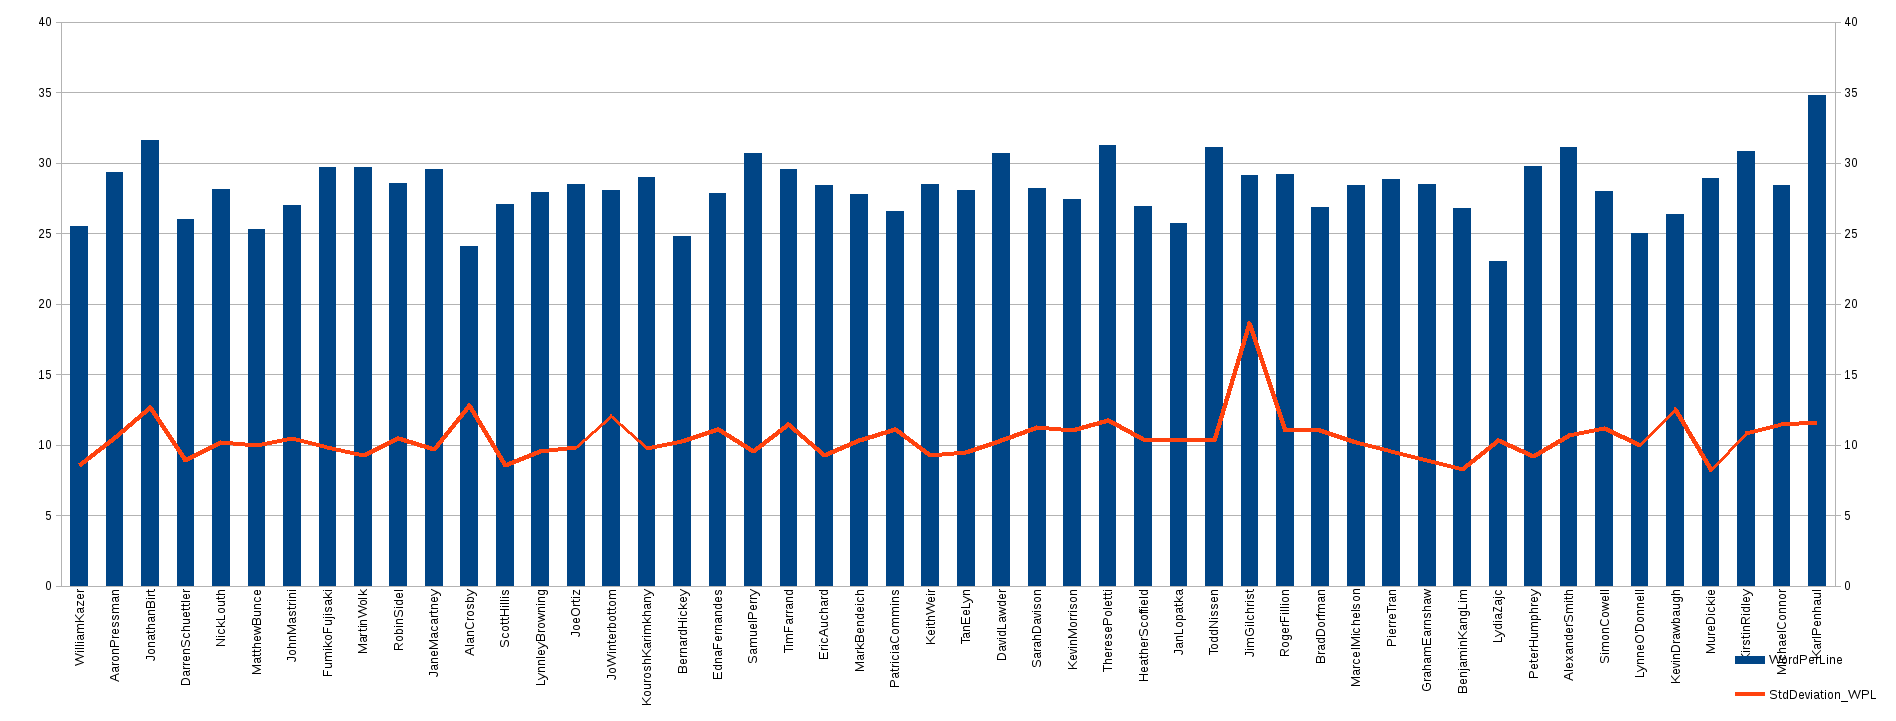
\includegraphics[width=11cm]{fig/WPL.png}
\caption{Mots par paragraphe}
\label{WPL}
\end{figure}

À ce stade, nous avons décidé de laisser de côté ces analyses trop simples. En effet, ces analyses se concentrant uniquement sur un élément particulier, les résultats ne peuvent être que dilués dans l'ensemble des données.

\todo{Changer : montrer que ce n'est pas discriminant}




\subsection{Étude des transitions}

Afin de parvenir à identifier les auteurs de nos textes, nous avons pensé qu'il serait plus judicieux de nous intéresser aux schémas apportés par les transitions. En effet, un auteur utilisant beaucoup de qualificatifs ou ayant une manière plus particulière d'exprimer les choses pourra potentiellement être identifié par ce biais là. C'est à ce moment là que nous nous sommes réellement posé la question de la pertinence de nos précédentes métriques. En effet, nos métriques précédentes ne sont-elles pas intrinsèques au langage ?

Par l'étude de la transition, nous avons souhaité construire assez simplement une matrice représentant tous les tags proposés par Tree Tagger et nous permettant de savoir si le tag X est suivi du tag Y.

\[M=\bordermatrix{
&TAG_{1}&\cdots&TAG_{j}&\cdots&TAG_{n}\cr
TAG_{1}& occ_{11} & \cdots & occ_{1j} & \cdots & occ_{1n} \cr
\vdots&\vdots&\ddots&\vdots&\ddots&\vdots\cr
TAG_{i}& occ_{i1} & \cdots & occ_{ij} & \cdots & occ_{in} \cr
\vdots&\vdots&\ddots&\vdots&\ddots&\vdots\cr
TAG_{m}& occ_{m1} & \cdots & occ_{mj} & \cdots & occ_{mn} \cr
}\]

Cette matrice n'apporte rien seule, notre idée ici était de mettre en place une analyse moins individuelle des schémas. Nous voulions être capable de nous abstraire un peu de nos tags pour nous consacrer plus sur le \textit{dessin} qui était créé par cette matrice. À ce stade, nous avons cherché quels étaient les outils que nous pouvions mettre en place pour parvenir à une telle analyse. Nous avons ainsi regardé différents algorithmes tels que ceux en rapport avec les matrices stochastiques, les algorithmes en rapport avec la théorie des graphes, etc. Une façon de procéder a retenu notre attention.

Cependant, ce qui a retenu notre attention ici sont deux expériences apportées par un membre de l'équipe dans l'étude de similitudes pour reconnaître des visages (eigenfaces\footcite{http://fr.wikipedia.org/wiki/Eigenface}) et une expérience similaire pour un tri de données spatialisées utilisant des matrices de covariance et des valeurs propres. Partant alors en quête d'une solution avec ces outils, nous avons tenté de mettre en place une méthode de comparaison matricielle en employant les vecteurs caractéristiques extrait de nos matrices.

Malheureusement, nous avons dû abandonné cette approche commençant à manquer de temps et sentant que nos connaissances auraient besoin d'être approfondies pour obtenir les prémices d'un résultat. Néanmoins, cette approche nous semble intéressante dans le sens où elle permet de s'abstraire des données originales et de plus se concentrer sur la forme du message. Nous avons réalisé ce début de prototype en Python en exploitant la bibliothèque \textit{numpy} et les algorithme fournis dans le package LAPACK\footcite{http://www.netlib.org/lapack/}.

\subsection{Déploiement de la méthode des N-grams}

L'étude des transitions nous ayant posé quelques problèmes pour trouver une manière élégante de comparer des matrices de transitions, nous nous sommes penchés sur une méthode un peu plus générique et nous offrant peut-être un peu plus de souplesse quant à sa configuration. Toujours dans l'idée d'identifier nos auteurs par leur façon de tourner leurs phrases, cette méthode nous permet de choisir la longueur de nos «~grams~» et d'en ressortir un résultat assez simplement.

Cette méthode nous permet de tirer partis de l'ordre dans lequel sont écris les mots utilisés par nos auteurs. Après avoir passé l'ensemble de notre corpus de test sous forme de tag, avec le même outil que précédemment (Tree Tagger), nous analysons les différents enchaînements de tags repérés dans nos fichiers. Pour un 2-grams, nous nous occuperons seulement des enchaînement de 2 tags, pour un 3-grams, des enchaînements de 3 tags, etc ...

Pour se faire, nous prenons un à un chacun des enchaînements que nous rencontrons, comptabilisons son nombre d'occurrence dans l'ensemble des articles d'un auteur, puis compilons ces résultats. Nous prenons également en compte que l'apparition d'un unique enchaînement dans l'ensemble du corpus n'est pas assez discriminant pour notre recherche : Il sera alors supprimé de notre comptabilisation. L'ensemble de ces calculs et mises en formes sont réalisés à l'aide de script perl, simplifiant la lecture et l'écriture au sein de fichiers .txt et .csv.

Suite à cette première analyse, un fichier .csv récapitulatif des fréquences d'apparition de ces suite est généré. Ce dernier, classé par auteurs, est ensuite comparé à notre fichier à classifier mis sous forme de tag et pré-analyser : est alors réalisé une comparaison point à point de l'ensemble des combinaisons liées à un auteur. Nous calculons son taux de "matching" et sortons l'auteur ayant le plus fort taux d'affiliation et donc, le plus probable pour ce texte. 

Cette méthode est tout de fois assez lourde puisqu'elle requiert une bonne dizaine de minute pour s'exécuter intégralement bien que déjà placée totalement en mémoire (sur un système de fichier tmpfs). 

Néanmoins, jusqu'à présent, seule cette méthode a réussi à nous montrer des résultats concret bien que décevant d'un point de vue qualitatif. Nous obtenons une variation de l'efficacité de cette méthode en fonction du nombre de mots pris en compte dans nos enchaînements :

\begin{itemize}
\item{Pour un 2-grams : nous obtenons environ 26\% de réussite.}
\item{Pour un 3-grams : nous descendons à une valeur de 21\% de réussite.}
\item{Pour un 4-grams : nous chutons à moins de 14\% de réussite}
\end{itemize}

Nous avons également tester des n-gramms prenant en compte plus de mots, mais ces derniers se sont révélés assez peu discriminant et donc inintéressant.



\section{Comparaison de performance}

Que ce soit la première méthode ou la seconde, nos résultats nous paraissent assez décevants. En effet, il nous est impossible d'identifier ne serait-ce que 50\% des textes convenablement. Néanmoins, voici un tableau récapitulant les performances obtenues sur les différents stades de deux méthodes développées.

\todo{Critiquer l'approche que l'on a eu, montrer les faiblesses}
\todo{Méth2: difficulter de différencier le style du langage (anglais)}

\todo{Insérer un tableau comparatif}

\begin{table}[H]
\centering
\begin{tabular}{|c|c|c|}
\hline 
 & \textbf{Term-frequency criterion} & • \\ 
\hline 
\textbf{Bien classé} & • & • \\ 
\hline 
\textbf{Mauvais classé} & • & • \\ 
\hline 
\textbf{Pas classé} & • & • \\ 
\hline 
\end{tabular} 
\caption{Résumé des performances des algorithmes}
\end{table}

%\begin{center}
%\begin{tikzpicture}[scale=1]
%\begin{axis} [ybar=1,xtick={1,2,3,4,5},nodes near coords, xticklabels={Sophie,Ginette,Robert,Roland,Marcel}]
%\addplot coordinates{(1,21)(2,2)(3,12)(4,5)(5,7.5)}; 
%\addplot coordinates{(1,5)(2,6)(3,9)(4,3)(5,10)};
%\addplot coordinates{(1,8)(2,2)(3,7)(4,5)(5,10)};
%\legend{Bien classés,Mal classés,Pas classés}
%\end{axis}
%\end{tikzpicture}
%\end{center}

En ce qui concerne la première méthode, ne s'agissant que d'un travail sur les mots les plus fréquents, il parait évident que cela ne va pas permettre d'obtenir un classement parfait, vu que nous sommes loins de prendre en compte toutes les finesses et les styles des auteurs. Cependant, il nous semblait que cela suffirait pour plus de situations. Nous sommes donc assez déçus du niveau de performance obtenu. D'autre part, nous avons trouvé la métrique utilisée dans la classification pas forcément appropriée, ce qui peut expliquer un taux de mauvais classés aussi important.


\section*{Conclusion}
\addcontentsline{toc}{section}{Conclusion}

\todo{Identification de nos erreurs, bilan technique et péda}
Ce projet nous a permis déjà de nous rendre compte du travail nécessaire à la réalisation d'algorithmes de classification, en particulier de la partie mathématique. Nous avons donc obtenu une certaine sensibilisation aux techniques utilisées au lieu d'être de simples consommateurs d'algorithmes comme nous l'avons été durant certains TPs en début de semestre. 

Nous pensons également que nos piètres résultats en terme d'efficacité sont sûrement dus à des erreurs ou des approximations mathématiques. \todo{à compléter}

\end{document}
